\chapter{Blockchain}

A blockchain is a fully-distributed, peer-to-peer software network which makes use of cryptography to securely host applications, store data and transfer digital assets that could represent real-world assets; this technology can be thought as a append-only master ledger that is publicly available and is not controlled by a central authority.\\

Blockchain systems, since 2008, year of Bitcoin white paper, have received a lot of attentions from whom is interested in building products and services and who want to invest in those assets.

Technically speaking a blockchain is a grown list of records, called blocks, which are linked using cryptographic techniques and widely used by cryptocurrencies.\\
There is no actually a formal definition of blockchain technology that is generally accepted but is possible to defined it using the Bitcoin as model and its application in cryptocurrencies.\\

Bitcoin's blockchain was presented by Sathosi Nakamoto in 2008 to solve the problem of building and using a decentralized protocol to implement digital currency without the need of a trusted authority or central server and avoid double-spending from malicious players. 

Banks should kepp track of all parties balances in a ledger that is not visible by the public. Banks system rely on trust: each party should trust the bank upon every transaction and the bank can decide to reject or accept it.\\
This centralization is the first aspect that lead to the implementation of first electronic payments based on cryptography techniques.

Another definition of blockchain is provided by Vitalik Buterin, co-founder of Ethereum:\newline

``A blockchain is a magic computer that anyone can upload programs to and leave the programs to self-execute, where the current and all previous states of every program are always publicly visible, and which carries a very strong cryptoeconomically secured guarantee that programs running on the chain will continue to execute in exactly the way that the blockchain protocol specifies.``\\

This definition is interesting since do not mention financial terms, particular use cases, specific consensus protocols or algorithms but do not take into consideration aspects like decentralization and communication.

\section{Structure}

A blockchain is commonly composed in:
\begin{itemize}
    \item Blocks
    \item Protocols
    \item Nodes
\end{itemize}

\subsection{Blocks}

A block in a single record that forms the growing list of records.

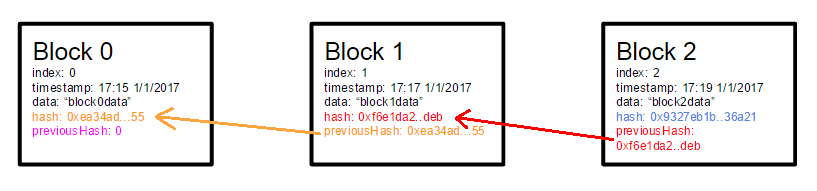
\includegraphics[scale=0.45]{images/blockchain_basic.png}

Blocks are linked using cryptography and by design are resistant to data modification. Cryptography provides authentication and verification and is used to conjure a secure computing environment out of many nodes without central authority or single owner.\\
Each block contains a cryptographic hash of the previous block, a timestap and the data to store in a permanent way.

Each block contains a cryptographic hash of the previous block,[6] a timestamp, and transaction data (generally represented as a merkle tree root hash). By design, a blockchain is resistant to modification of the data. It is "an open, distributed ledger that can record transactions between two parties efficiently and in a verifiable and permanent way".[8] For use as a distributed ledger, a blockchain is typically managed by a peer-to-peer network collectively adhering to a protocol for inter-node communication and validating new blocks. Once recorded, the data in any given block cannot be altered retroactively without alteration of all subsequent blocks, which requires consensus of the network majority.

Though blockchain records are not unalterable, blockchains may be considered secure by design and exemplify a distributed computing system with high Byzantine fault tolerance. Decentralized consensus has therefore been claimed with a blockchain.[9]

Blockchain was invented by Satoshi Nakamoto in 2008 to serve as the public transaction ledger of the cryptocurrency bitcoin.[1] The invention of the blockchain for bitcoin made it the first digital currency to solve the double-spending problem without the need of a trusted authority or central server. The bitcoin design has inspired other applications.[1][3]
Qui una breve descrizione del contenuto del capitolo o, eventualmente, testo introduttivo alle sezioni che seguono

\section{Prima Sezione}
Qui il testo della prima sezione. Questa è  una parola in \textit{corsivo}, questa invece è una parola in \textbf{grassetto} e questa è una parola in \texttt{monotype}.

\begin{center}
Questo è un paragrafo centrato!
\end{center}

Dimensione del testo:\\

\LARGE{Testo} \Large{Testo} \large{Testo} \normalsize{Testo} \small{Testo} \footnotesize{Testo}\\

Qui una citazione bibliografica \cite{bib001}.

Qui un link \url{www.google.it}


\subsection{Prima Sottosezione}

Qui l'esempio di un elenco puntato:

\begin{itemize}
\item Primo elemento,
\item Secondo elemento,
\item Terzo elemento.
\end{itemize}

Qui l'esempio di un elenco con un sotto-elenco:

\begin{itemize}
\item Primo elemento,
\begin{itemize}
\item Primo elemento del sotto-elenco
\item Secondo elemento del sotto-elenco
\end{itemize}
\item Secondo elemento,
\item Terzo elemento.
\end{itemize}

Qui infine l'esempio di un elenco numerato

\begin{enumerate}
\item Testo
\item Testo
\item Testo
\end{enumerate}

\section{Seconda Sezione}\label{sec:Sezione2}

Qui l'esempio di una formula matematica:

$ G = \gamma\dfrac{m_{1}m_{2}}{r^{2}} $

\section{Terza Sezione}

Qui il riferimento ad una sezione utilizzando una label: Sezione \ref{sec:Sezione2}

Qui la definizione di due paragrafi con titoli.

\paragraph{Titolo 1} testo del paragrafo

\paragraph{Titolo 2} testo del paragrafo, con una nota a piè di pagina\footnote{Questo è il testo della nota, in cui si può \textit{utilizzare} qualunque stile di \textbf{formattazione}}

